% !TEX root = ../Thesis.tex
\chapter{Superpage Overlay Design}

To identify which parts of a superpage are mapped to an overlay, the OBitVector is appended to the TLB entries for superpages. On a TLB hit for a 2MB superpage, the lower-order bits of the address are used to check the corresponding index in the OBitVector. If it is 0, the translation is returned as normal. If it is 1, the 4KB TLB is checked instead. On a TLB miss in this situation, the memory controller can proceed directly to the Overlay Mapping Table (OMT), since there is guaranteed to be an overlay for this address.

The OMT is simply a secondary page table hierarchy, which maps virtual addresses that have overlays to the physical address of the overlay page. The OBitVector for an address is implicitly included in the OMT: an address not present at the 2MB level of the OMT is has an all-zero OBitVector, and otherwise it consists of the present bits of the next level page table. On a TLB miss of any kind, the memory controller walks the regular page table as normal. Concurrently, it walks the OMT and overrides the mapping if the address is present there. Both the superpage translation from the standard page table and the small page translation from the OMT are then cached in the TLB, along with the computed OBitVector.

\section{Performance Impact}
In the case of a hit in the 2MB TLB, performance will be only very slightly impacted by the requirement of testing one additional bit. Hits in the 4KB TLB are completely unchanged. Since the two sets of TLB entries can be queried concurrently, there is no extra impact from an address that is present in both TLBs. Thus, in the common case superpage overlays do not hurt performance, and the increased TLB reach offered by better superpage utilization makes that case even more common.

The page table walk is complicated by the requirement of walking an additional page table hierarchy, but the two operations can be done concurrently and the OMT walk will quickly stop in the common case where there are no overlays. Page table walks for superpages (when the address doesn't have an overlay) still take three sequential memory accesses compared to four for a small page or overlay, so that benefit over small pages is retained.

Calculation of the OBitVector for pages that have overlays incurs a substantial cost, since the first bit of each PTE must be read. This adds 511 extra memory accesses to a page table walk when the address is a superpage with overlays, though they are sequential so they should have good cache behavior. There is also increased cache pressure because there are simply more page tables to cache. Again, making page table walks less common should offset that cost.

\section{Possible Variants}
The above outlines the simplest version of the superpage overlay framework, which just adds OBitVectors to the 2MB TLB and an additional page table hierarchy that is no different from the existing one. There are three variants that could improve the performance of the modified page table walk at the cost of greater page table and memory controller complexity.

The simplest one is to store the OBitVector directly in the 2MB level of the OMT rather than building it by examining the present bits of the next level table. This makes the table take up multiple pages of memory, since more information must be stored per entry. It would yield a significant performance improvement to the OMT walk, since the last pointer need not be followed when there is no overlay and the OBitVector need not be calculated from multiple memory accesses.

The second variant is storing the OBitVector in the regular page table instead of the OMT, which allows the OMT walk to not occur at all in the common case. Altering the structure of the existing page table is a much greater cost than altering the newly proposed OMT, however. Reducing the number of entries per page table or increasing the size of a page table would have significant consequences.

Finally, both the OBitVector and the overlay mappings could be stored directly in the 2MB level of the regular page table. In other words, each entry would include the physical address of a superpage, the OBitVector, and the physical address of a page table for the 4KB entries. This eliminates the OMT altogether, and the page table walk just stops at the 2MB level like a regular superpage or continues to the 4KB level like a regular page depending on the OBitVector test. That would result in almost no performance impact on the page table walk, but increasing the size of page table entries by that much would likely hurt performance in other areas too greatly.

All three of these variants could be tuned by using a smaller OBitVector where each bit applies to multiple 4KB pages. This reduces the flexibility improvements because superpages can only be managed at the granularity that the OBitVector allows, but it reduces the impact on the size of page table entries.

These implementation details are not further covered in this paper because our evaluation of superpage overlays is based on a simulation framework that does not model page table changes at that level of detail.

\section{Hardware Cost}
Enabling superpage overlays requires changing the hardware in the TLB and the MMU, but the changes are relatively simple. A bit vector must be added to each 2MB TLB entry (64 bytes per entry), and the logic for a TLB hit changed to test the bit vector and defer to the 4KB TLB for overlays. The MMU must be modified to walk the OMT along with the regular page tables, but the OMT is essentially the same as a regular page table so the cost should be relatively low. Finally, a special-purpose register is needed to store the process-specific OMT address, just like the existing CR3 register.

\section{Using Overlays}
Utilizing the superpage overlay system is up to the operating system. The OMT can be managed in the same way as regular page tables.

\subsection{Overlay-on-Write}
The main application of superpage overlays presented is overlay-on-write. This changes the copy-on-write policy for superpages to avoid copying the entire superpage. In existing systems, when a process is forked the new process maps to the same physical pages as the parent, and all writable pages are marked read-only for COW. When a write is made to a superpage marked for COW, the whole page is copied and the page table for the writing process is updated to point to the new superpage. With overlay-on-write, only the 4KB section of the superpage that is written is copied, and that new page is added to the OMT for the writing process. Figure \ref{fig:oow} visualizes the difference. As a result, much less data is copied if the processes only change a small portion of their writable pages. If a part of a superpage that already has an overlay must be copied, it can be treated exactly the same as a regular small page.
\begin{figure}
    \centering
    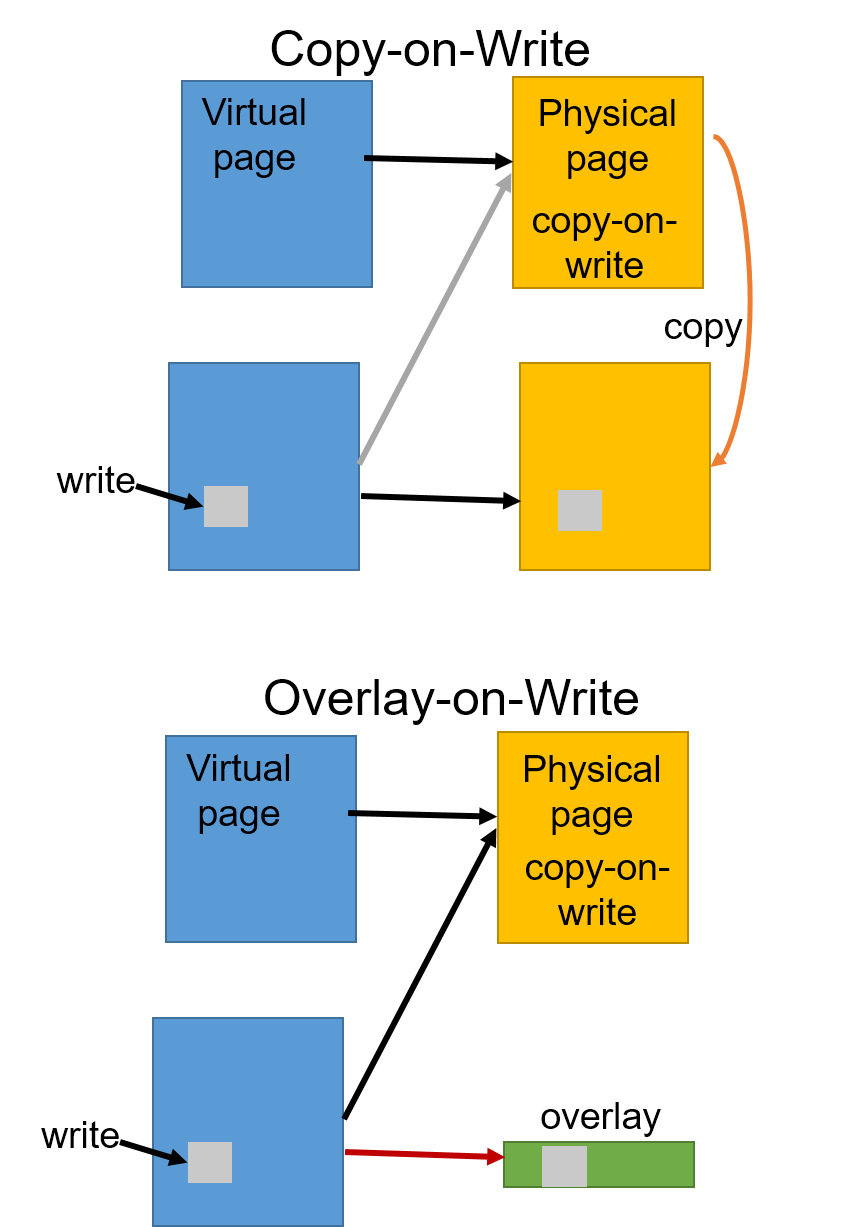
\includegraphics[width=2in]{Figures/Picture2}
    \caption{The difference between copy-on-write and overlay-on-write}
    \label{fig:oow}
\end{figure}

\subsection{Memory Checkpointing}
In addition to making the fork operation inexpensive, overlay-on-write can be used for memory checkpointing. A simple approach to fault tolerance is making backups of the entire address space at regular intervals, which can be restored if anything goes wrong.

The goal of a memory checkpointing system is to take a snapshot of the full contents of the address space at a moment in time, and copy it to some form of nonvolatile memory to be used as a backup. To do this, all writable addresses are marked for COW when the checkpoint starts. This is essentially the same as a fork operation, except that the child process is a special checkpoint thread controlled by the kernel. From the checkpoint thread's point of view, the memory becomes fixed at the moment the checkpoint started, even though the main processes continues running. The checkpoint thread simply iterates through the address space, copies pages to some form of nonvolatile memory, and removes the COW designation on each page it finishes processing. The same overlay-on-write logic applies so that the program can continue utilizing superpages while the checkpoint is in progress without having to COW 2MB at a time.

There is another similar use of memory checkpointing, which facilitates transactional operations. The checkpoint is again a snapshot of memory at a moment in time, but rather than being copied to nonvolatile memory it is simply kept in main memory while the program continues to execute. Then, when the program reaches a certain point the changes it has made since the previous snapshot are ``committed'' and become the next snapshot. The enables the execution of the program to be rolled back to the previous commit if an error occurs or the transaction is canceled by reverting every page to the snapshot version.

\subsection{Overlay Switching}
With memory checkpointing, checkpoints will be taken repeatedly at regular intervals. This means superpages will be marked COW repeatedly, and the number of pages in overlays will increase. If most of a superpage has overlays, the benefits of the superpage are lost and we only have the downsides of the OMT walk. Thus, we want to limit how many overlays a superpage can have.

To facilitate that, when an overlay-on-write occurs the OS should attempt to allocate the new pages in their proper alignment within a ``reserved'' superpage. This reservation can easily be tracked in a kernel data structure. Then, when more than half of the superpage has overlays, the OMT and regular page table entries can be swapped so that the aligned overlays form a new superpage and the parts of the original that were not copied become overlays. No flexibility is lost, since other overlays not in the reserved superpage can still be retained. Assuming that there is a free 2MB aligned region to reserve and that checkpointing is the only source of overlays, this means any superpage will have at most 256 overlays and thus will retain most of the superpage benefits no matter how many checkpoint iterations occur.

\subsection{Superpage Coalescing}
Prior works like GLUE \cite{Pham} and SpecTLB \cite{Barr} focus on creating speculative superpages by identifying regions of memory that are mostly aligned to a 2MB boundary. This is more flexible in some ways than simply preserving superpages that already exist and would otherwise be split. The superpage overlay system can identify and coalesce mostly-aligned superpages in software by extending the existing THP daemon in Linux. The daemon periodically scans memory for small pages that form a fully aligned 2MB region (with the same permission bits) and merges them into a superpage \cite{THP}. With superpage overlays, the daemon can be modified to simply scan for and merge 2MB regions in which more than half of the small pages are aligned to the same physical region. Any unaligned small pages then become overlays. The number of small pages that must be aligned for a superpage to be created could be tuned, and the OS could even use some heuristic based on how volatile the memory region is.

\subsection{Overlay Resetting}
Finally, sometimes a superpage may have to become mostly covered by overlays. When this happens, it is best to remove the superpage and turn it into regular small pages. This is very easy to do: simply fill in the missing entries in the last-level OMT and point the regular page table to it. Since most of the OMT entries already exist, this is less expensive than a single page copy. Like coalescing, this operation can easily be tuned in terms of when a superpage is reset. The OS could have some heuristic that determines how much activity is in the overlays versus the non-overlay parts of the superpage, and decide when to reset based on that.
